\documentclass[tikz,border=12pt]{standalone}
\usepackage{amsmath,amssymb}
\usetikzlibrary{calc,arrows.meta}

\begin{document}
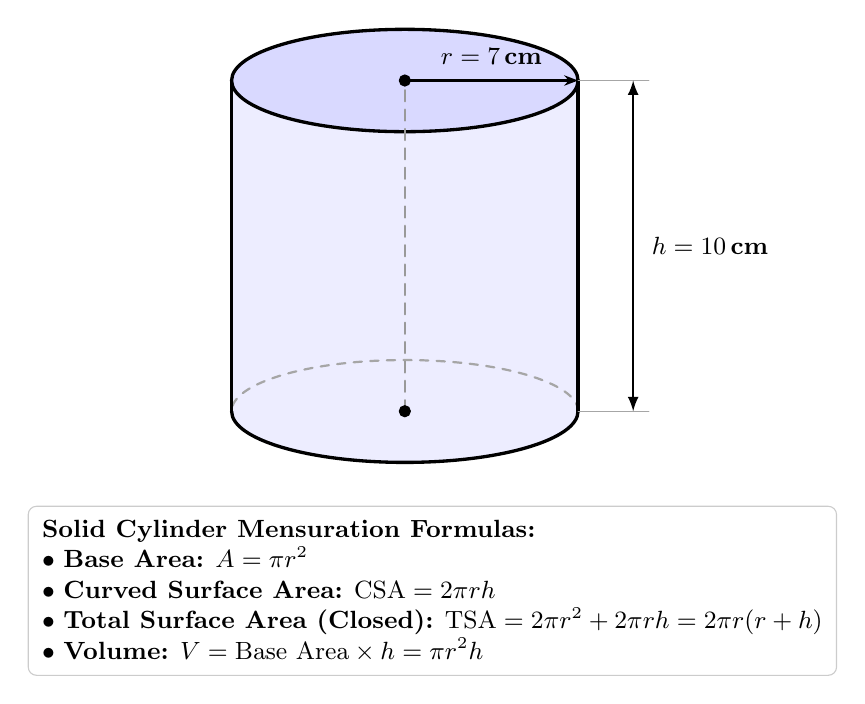
\begin{tikzpicture}[>=latex, line cap=round, line join=round]

  % Geometric parameters
  \def\rx{2.2}
  \def\ry{0.65}
  \def\h{4.2}

  % Cylinder body shading
  \fill[blue!7] (-\rx, 0) arc (180:360:\rx cm and \ry cm) -- (\rx, \h) arc (0:180:\rx cm and \ry cm) -- cycle;

  % Hidden bottom ellipse (dashed)
  \draw[thick, dashed, gray!70] (\rx, 0) arc (0:180:\rx cm and \ry cm);

  % Visible bottom ellipse (solid)
  \draw[very thick] (-\rx, 0) arc (180:360:\rx cm and \ry cm);

  % Vertical contours (left and right edges)
  \draw[very thick] (-\rx, 0) -- (-\rx, \h);
  \draw[very thick] (\rx, 0) -- (\rx, \h);

  % Top ellipse (solid, shaded slightly lighter)
  \fill[blue!15] (0, \h) ellipse (\rx cm and \ry cm);
  \draw[very thick] (0, \h) ellipse (\rx cm and \ry cm);

  % Central vertical axis (dashed)
  \draw[thick, dash pattern=on 4pt off 3pt, gray!80] (0, 0) -- (0, \h);

  % Center point on top base
  \filldraw[black] (0, \h) circle (2pt);
  \filldraw[black] (0, 0) circle (2pt);

  % Radius callout on top face
  \draw[thick, -{Stealth[length=5pt]}] (0, \h) -- (\rx, \h) node[midway, above=2pt, font=\small\bfseries] {$r = 7\,\text{cm}$};

  % Height callout with extension lines on right
  \draw[thin, gray!70] (\rx, \h) -- (\rx + 0.9, \h);
  \draw[thin, gray!70] (\rx, 0) -- (\rx + 0.9, 0);
  \draw[thick, <->] (\rx + 0.7, 0) -- (\rx + 0.7, \h) node[midway, right=3pt, font=\small\bfseries] {$h = 10\,\text{cm}$};

  % Mensuration Formula Card below
  \node[align=left, font=\small, fill=white, inner sep=5pt, draw=gray!40, rounded corners=3pt, anchor=north] at (0.35, -1.2) {
    \textbf{Solid Cylinder Mensuration Formulas:}\\
    $\bullet$ \textbf{Base Area:} $A = \pi r^2$\\
    $\bullet$ \textbf{Curved Surface Area:} $\text{CSA} = 2\pi r h$\\
    $\bullet$ \textbf{Total Surface Area (Closed):} $\text{TSA} = 2\pi r^2 + 2\pi r h = 2\pi r(r + h)$\\
    $\bullet$ \textbf{Volume:} $V = \text{Base Area} \times h = \pi r^2 h$
  };

\end{tikzpicture}
\end{document}
